%Plataformas de pesquisa. Strings de busca avançada. Buscadores de periódicos.

\section{``Estado-da-arte'' x ``Estado da arte''}

\begin{frame}{História}
\begin{itemize}
\item No século XIX, \emph{estado da arte} tinha o sentido de \emph{status da arte}, i.e. ``o nível atual que alguma arte técnica havia alcançado''.
\item No início do século XX, passou a ter o sentido de ``estágio atual de desenvolvimento de um assunto prático ou tecnológico'', talvez por um engano da loquacidade.
\item A partir da segunda metade do século XX, a forma hifenizada \emph{estado-da-arte} passou a ser usada no sentido de ``a técnica mais recente ou melhor existente em algum produto ou atividade''.
\end{itemize}
\end{frame}

%%
\begin{frame}
\begin{itemize}
\item Para a escrita científica, a forma atual mais coerente seria: ``estado-da-arte'' (\emph{state-of-the-art}).
\item Em suma, ``o maior nível de desenvolvimento de um dispositivo, técnica ou campo científico atingido até então''
\item Sinônimos: ``fronteira do conhecimento'' (\emph{cutting edge}), ``vanguarda do conhecimento'' (\emph{leading edge})
\end{itemize}
Baseado em: \scriptsize{\url{https://english.stackexchange.com/questions/217898/how-when-and-where-did-the-phrase-state-of-the-art-originate}}
\end{frame}

%%
\begin{frame}{A escolha de um tópico de pesquisa}
\begin{itemize}
\item \textbf{Conheça a literatura:} tenha certeza de que suas contribuições serão novas e úteis
\item \textbf{Conheça a comunidade:} artigos provêm de desenvolvimentos contínuos. Entenda o que a comunidade faz para saber o que ela faz e saber como conversar com ela
\item \textbf{Pense grande:} tente resolver um ``grande problema'', ainda que tenha que andar passo a passo
\end{itemize}
\end{frame}

\begin{frame}
\begin{itemize}
\item \textbf{Gaste um tempinho:} boas idéias de pesquisa não acontecem todos os dias... Pode levar tempo, mas seus resultados serão mensurados pelo impacto, não pelo tempo que você levou para achar a idéia
\item \textbf{Não construa problemas que não existem:} apresentar um problema novo é legal, mas esteja certo de que é um problema realista. Se você não puder exemplificá-lo, ele provavelmente não é realista. 
\end{itemize}
Baseado em: Dredze \& Wallach
\end{frame}

\section{Bases de pesquisa}

%%
\begin{frame}{CAPES Periódicos}
\begin{itemize}
\item Criado em 1990 
\item Acesso garantido pela CAFe (Comunidade Acadêmica Federada), oferecida pela Rede Nacional de Ensino e Pesquisa (RNP)
\item Um custo milionário com assinaturas... R\$ 402 mi em 2017
\item Um portal a ser valorizado enquanto ele durar...
\item A tendência \emph{Open Access} poderá mudar o quadro em alguns anos...
\end{itemize}

Ver: \scriptsize{\url{https://www1.folha.uol.com.br/ciencia/2018/10/ciencia-europeia-tera-de-ser-publicada-em-revistas-de-acesso-livre-em-2020.shtml}}
\end{frame}

%%
\begin{frame}{O portal tem um aplicativo}
\begin{figure}

\includegraphics[scale=0.4]{figs/04/periodicos}
\quad
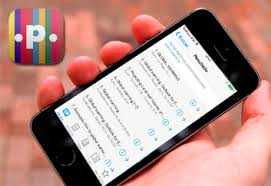
\includegraphics[scale=0.45]{figs/04/app}
\end{figure}

Disponível para iOS, Android e outras plataformas.\footnote{}
\end{frame}

%%
\begin{frame}{O problema da pesquisa paga...}
\begin{figure}
\centering
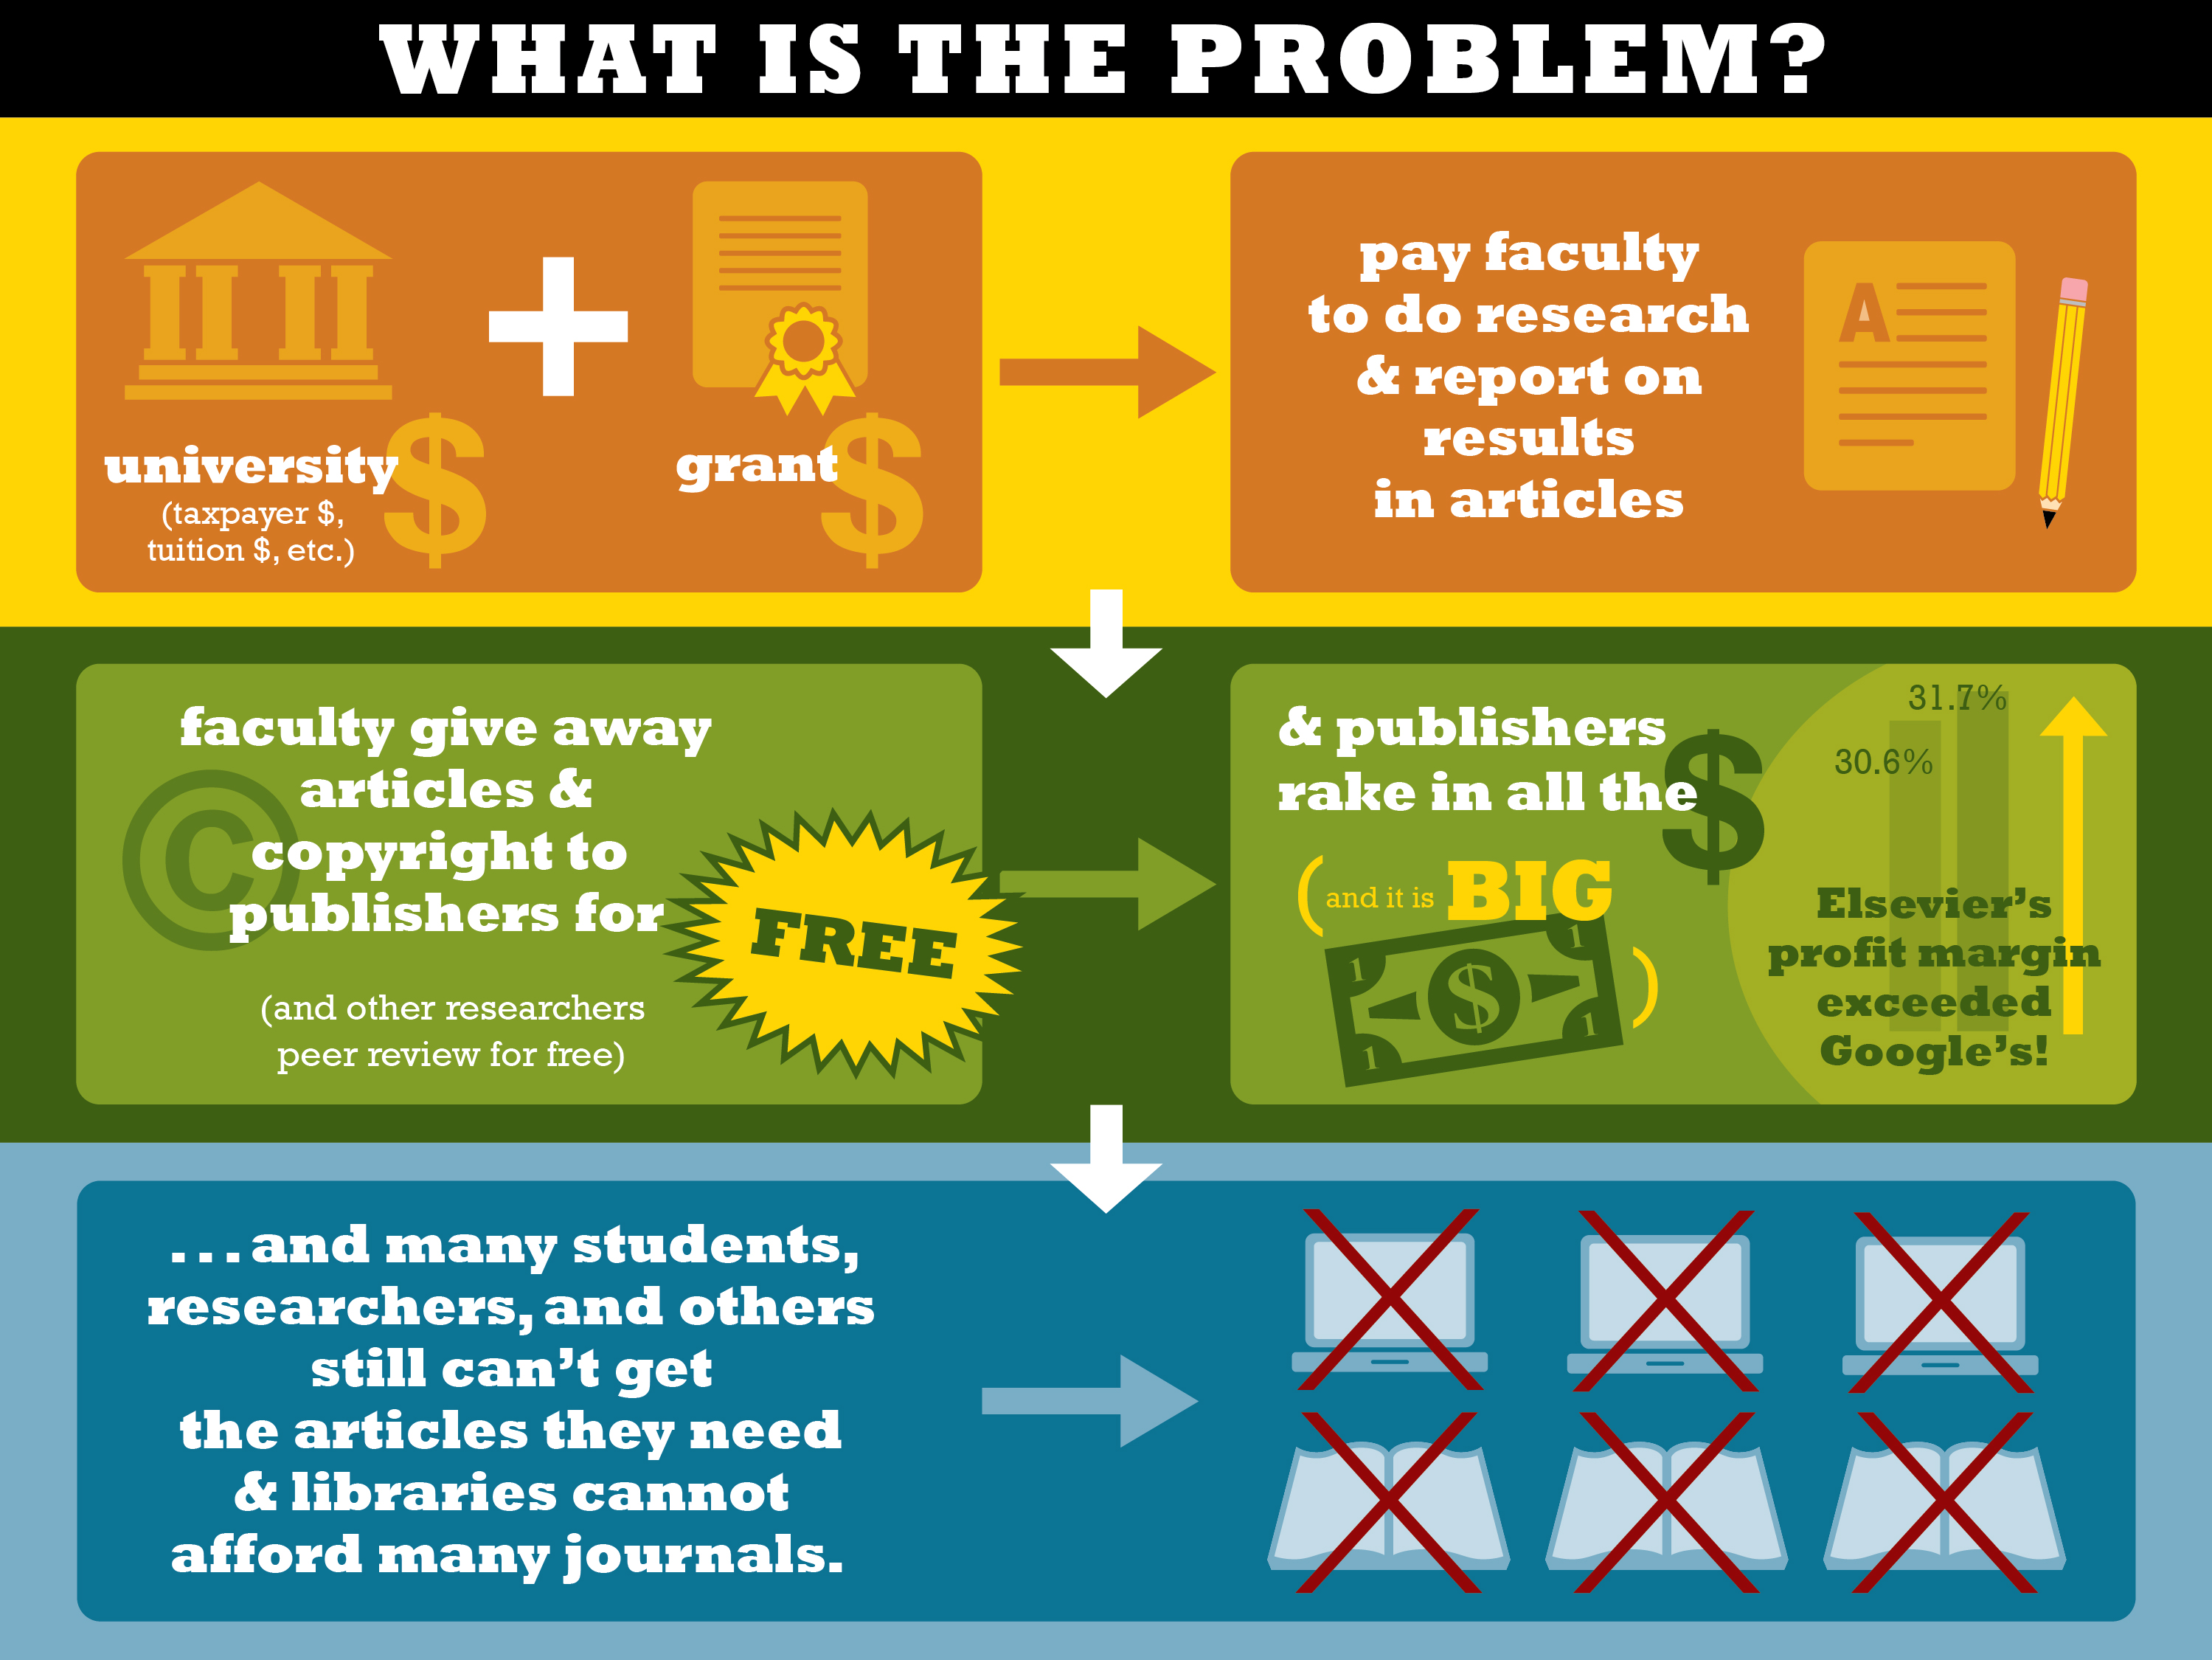
\includegraphics[scale=0.3]{figs/04/problem}
\caption{\scriptsize{Fonte: http://justpublics365.commons.gc.cuny.edu/files/2014/10/Problem-infographic3.jpg}}
\end{figure}
\end{frame}

%%
\begin{frame}{Open Access}
\begin{figure}

\includegraphics[scale=0.3]{figs/04/oa}
\end{figure}
\begin{itemize}
\item Mecanismo de distribuição da pesquisa científica de modo aberto e livre de custos
\item Veja o \emph{Open Access Book}\footnote{\url{https://cyber.harvard.edu/hoap/Open_Access_(the_book)}}
\item Veja o DOAJ - Directory of Open Access Journals\footnote{\url{https://doaj.org}}
\end{itemize}
\end{frame}

%%
\begin{frame}{Scielo}
\begin{figure}

\includegraphics[scale=0.4]{figs/04/scielo}
\end{figure}
\begin{itemize}
\item A \emph{Scientific Electronic Library Online - SciELO} é uma biblioteca eletrônica de acesso aberto para periódicos nacionais
\item Projeto conduzido pela FAPESP desde 2002
\item Na Eng. Mecânica, o JBSME foi descontinuado em 2012
\item Portal possui pouca oferta em relação à Eng. Mecânica 
\end{itemize}
\end{frame}

%%
\begin{frame}{Google Acadêmico \emph{(Google Scholar)}}

\begin{itemize}
\item Motor de busca online para (quase tudo) na literatura acadêmica
\item Supostamente o maior banco de dados de todos: 389 mi de documentos
\item Aberto e disponível em: \url{http://scholar.google.com.br} (versão em inglês é mais completa)
\item Sobre: \url{https://scholar.google.com.br/intl/pt-BR/scholar/about.html}
\end{itemize}
\scriptsize{\url{Ver: https://link.springer.com/article/10.1007{\%}2Fs11192-018-2958-5}}
\end{frame}

\subsection{\emph{Strings} de busca}

\begin{frame}{Voltando ao CAPES Periódicos}
\begin{itemize}
\item Acessando novamente as bases Scopus e Web of Science...
\item 1o. treinamento: Scopus
\end{itemize}
\end{frame}

\subsubsection{Treinamento: base Scopus}

%%
\begin{frame}{Mecanismos para busca avançada}
Baseado no \textit{Scopus Help}
\begin{itemize}
\item Operadores booleanos
\item Operadores de proximidade
\item Códigos de campo 
\item Caracteres curinga e especiais
\end{itemize}
\end{frame}

%%
\begin{frame}{Operadores booleanos}
\begin{block}{\texttt{OR}(OU)}
Pelo menos um termo deve aparecer
\end{block}
\begin{block}{Exemplo}
\texttt{writing OR style}
\end{block}
\begin{block}{Opções de busca}
Campos: Título, resumo, keywords (TITLE-ABS-KEY) \\
Intervalo de busca: 2015 - presente \\
Tipo de documento: \emph{Article or Review} \\
Tipo de acesso: All (todos) 
\end{block}
\begin{block}{Resultados}
\textbf{120.517} documentos!
\end{block}
\end{frame}

%%
\begin{frame}
\begin{block}{\texttt{AND}(E)}
Ambos os termos devem aparecer
\end{block}
\begin{block}{Exemplo}
\texttt{writing OR style AND conciseness}
\end{block}
\begin{block}{Opções de busca}
Campos: Título, resumo, keywords (TITLE-ABS-KEY) \\
Intervalo de busca: 2015 - presente \\
Tipo de documento: \emph{Article or Review} \\
Tipo de acesso: All (todos) 
\end{block}
\begin{block}{Resultados}
\textbf{30} documentos!
\end{block}
\end{frame}

%%
\begin{frame}
\begin{block}{\texttt{AND NOT}(E (``mas'') NÃO)}
Exclui um termo
\end{block}
\begin{block}{Exemplo}
\texttt{writing OR style AND conciseness AND NOT short}
\end{block}
\begin{block}{Opções de busca}
Campos: Título, resumo, keywords (TITLE-ABS-KEY) \\
Intervalo de busca: 2014 - presente \\
Tipo de documento: \emph{Article or Review} \\
Tipo de acesso: All (todos) 
\end{block}
\begin{block}{Resultados}
\textbf{28} documentos!
\end{block}
\end{frame}

%%
\begin{frame}{Ordem de precedência}
O motor de busca usará a seguinte ordem de precedência
\begin{enumerate}
\item \texttt{OR} 
\item \texttt{AND} 
\item \texttt{AND NOT}  (deve ser usado por último!)
\end{enumerate}
\begin{itemize}
\item Para buscar frases específicas, use aspas duplas (e.g. ``scientific writing'')
\item Para buscar por frases exatas, use chaves (e.g. \{scientific writing should be concise\})
\end{itemize}
\end{frame}

%%
\begin{frame}
\begin{block}{Exemplo}
\texttt{ \{scientific writing should\} AND concise OR easy AND NOT long}
\end{block}
\begin{block}{Opções de busca}
Intervalo de busca: 2015 - presente \\
Campos: todos (\emph{All fields}) \\
Tipo de documento: \emph{Article or Review} \\
Tipo de acesso: All (todos) 
\end{block}
\begin{block}{Resultados}
\textbf{1} documento! \\
\textit{Scientific writing as an art: An overview}, Sreeja et al. Int. J. of Current Pharmaceutical Review and Research, Volume 8, Issue 2, 2016, pp. 1-4.
\end{block}
\end{frame}

%%
\begin{frame}{A \textit{string} completa}
\begin{block}
\texttt{ALL ( \{scientific writing should\}  AND  concise  OR  easy  AND NOT  long )  AND  DOCTYPE ( ar  OR  re )  AND  PUBYEAR  >  2014 }
\end{block}
\end{frame}


%%
\begin{frame}{Operadores de proximidade}
\begin{block}{\texttt{W/n}}
Indica distância de \texttt{n} palavras, mas não a ordem (en. \textit{within}). 
O número \texttt{n} deve ser um inteiro de 0 a 255.
\end{block}
\begin{block}{Exemplo}
\texttt{conciseness W/10 writing} \\
`conciseness'' distante de ``writing'' por até 10 palavras
\end{block}
\begin{block}{Opções de busca}
Intervalo de busca: 2015 - presente \\
Tipo de documento: \emph{Article or Review} \\
Tipo de acesso: All (todos) 
\end{block}
\begin{block}{Resultados}
\textbf{7} documentos!
\end{block}
\end{frame}

%%
\begin{frame}{}
\begin{block}{\texttt{PRE/n}}
Indica que os termos devem aparecer em uma ordem específica de precedência (en. \textit{precedence})
\end{block}
\begin{block}{Exemplo}
\texttt{understandable PRE/25 writing} \\
Busca texto em que ``understandable'' precede ``writing'' por até 30 palavras
\end{block}
\begin{block}{Opções de busca}
Intervalo de busca: 2010 - presente \\
Tipo de documento: \emph{Article or Review} \\
Tipo de acesso: All (todos) 
\end{block}
\begin{block}{Resultados}
\textbf{33} documentos!
\end{block}
\end{frame}

%%
\begin{frame}{cont.}
\begin{itemize}
\item A mesma pesquisa anterior com a palavra \texttt{unambiguous} gera \textbf{9 resultados}
\item A mesma pesquisa anterior com a palavra \texttt{intelligible} gera \textbf{19 resultados}
\item A mesma pesquisa anterior com a palavra \texttt{comprehensible} gera \textbf{20 resultados}
\item A mesma pesquisa anterior com a palavra \texttt{clear} gera \textbf{1049 resultados}
\end{itemize}

Ou seja, na literatura técnica, sinônimos são usados, mas predominam as palavras menos rebuscadas. Por outro lado, o uso dessas palavras incomuns faria com que seu trabalho se destacasse?
\end{frame}

%%
\begin{frame}{Códigos de campo}
\begin{itemize}
\item Códigos de campo são strings de busca formadas por campos predefinidos 
\item O Scopus possui mais de 60 campos 
\end{itemize}
\end{frame}


%%
\begin{frame}{Campos mais utilizados}
\begin{itemize}
\item \texttt{TITLE}; 
\item \texttt{TITLE-ABS-KEY}: título + resumo + palavra-chave
\item \texttt{AF-ID}: identificador da instituição do autor (no. definido pelo Scopus)
\item \texttt{AU-ID}: identificador do autor (no. definido pelo Scopus)
\item \texttt{ORCID}: ORCID do autor
\item \texttt{KEY}: palavra-chave
\item \texttt{ISSN}: número serial de publicação
\item \texttt{REF}: campo combinado para buscar referências
\end{itemize}
\end{frame}

%%
\begin{frame}{Exemplos}
\begin{itemize}
\item \texttt{TITLE(``scientific writing'')}: 
\item \texttt{TITLE-ABS-KEY(``academic style'')}
\item \texttt{AF-ID(Harvard Medical School 3000604)}
\item \texttt{AU-ID(100038831)} 
\item \texttt{ORCID(``0000-0002-1108-3360'')}
\item \texttt{KEY(style)}
\item \texttt{ISSN(0-7623-106)}
\item \texttt{REF(darwin 1859)}: ocorrem na mesma referência
\item \texttt{REF(darwin) AND REF(1859)}: no mesmo documento, mas não na mesma referência
\end{itemize}
\end{frame}

%%
\begin{frame}
\begin{block}{Exemplo}
\texttt{TITLE-ABS ( "graduate" )  AND  KEY ( efficiency )  AND  REF ( {scientific writing} ) }
\end{block}
\begin{block}{Opções de busca}
Query string pura
\end{block}
\begin{block}{Resultados}
\textbf{1} documento!
\textit{Supporting the writing productivity of biomedical graduate students: An integrated, structured writing intervention}, Gardner, S.A et al., Life Sciences Education, Vol. 17, Issue 3, 2018 (Open Access)
\end{block}
\end{frame}


%%
\begin{frame}{Caracteres curingas (\textit{Wildcards})}
Há duas formas de buscar por frases: busca exata e busca aproximada

\begin{itemize}
\item Buscas exatas são feitas com aspas ou chaves como já dissemos 
\item Buscas aproximadas não requerem aspas ou chaves 
\item Caracteres curingas podem ser incorporados às buscas para ampliar ou reduzir a busca
\end{itemize}
\end{frame}

\begin{frame}{Exemplos}
\begin{itemize}
\item \texttt{well-written} ou \texttt{well written} retornam o mesmo
\item \texttt{``well-written''} e \texttt{``well written''} retornam coisas diferentes
\item \texttt{sci* wr*} pode retornar ``science writing'', ``scientific writing`` ou ``science wrote``, ou mesmo ``scissor wrecking'' (se é que faz sentido)
\item \texttt{``sci* writing''} pode retornar ``science writing'', ``scientific writing`` ou ``sci-tech writing''
\end{itemize}
\end{frame}

\begin{frame}{Exemplos}
\begin{itemize}
\item O hífen é ignorado a menos que faça parte de uma frase exata
\item O ``*'' é ignorado quando precedido por hífen que é precedido por uma palavra:
\texttt{ABS(sci-*)} terá o mesmo efeito que \texttt{ABS(sci)}
\end{itemize}
\end{frame}

\begin{frame}{\emph{Stop words}} 
\begin{itemize}
\item Aspas duplas servem para fazer buscas específicas incluindo as chamadas \emph{stop words}
\item Por exemplo: \texttt{``writing with style''} pode retornar frases como \texttt{``writing with style is great skill''} 
\item \texttt{writing with style} ignorará ``with'' por ser uma \emph{stop word}
\end{itemize}
\end{frame}

\begin{frame}{Lista das \emph{Stop words}} 
Várias palavras são \textbf{ignoradas} nas buscas feitas pelo Scopus, a menos que incluídas em busca exata (com aspas ou chaves)-
\begin{itemize}
\item Pronomes pessoais (e.g. \emph{we}, \emph{they})
\item Artigos definidos e indefinidos (e.g. \emph{the}, \emph{an})
\item A maioria das formas do verbo \textit{to be} (e.g. \emph{be}, \emph{being}, \emph{is}, \emph{was})
\item Algumas conjunções (e.g. \emph{as}, \emph{because}, \emph{if}, \emph{when})
\end{itemize}
\end{frame}

\begin{frame}{Outras \emph{Stop words}} 
\begin{itemize}
\item about, again, all, also, because
\item due, done, does , how, itself, just
\item mainly, on, rather, show 
\item than, that, to, when, which, would
\item Existem mais... 
\end{itemize}

Eis um motivo para evitar muitas \emph{stop words} em títulos de artigo. Não servem para indexação...
\end{frame}

\subsubsection{Treinamento: base Web of Science}

%%
\begin{frame}{Mecanismos para busca avançada}
Baseado no \textit{Web of Science's Search Tips}\footnote{Os mecanismos de busca da WoS possuem muitas similaridades com aqueles da base Scopus no que tange à formação das strings de busca. Logo, é suficiente entender a lógica das strings de busca e aplicá-la a cada base convenientemente.}
\begin{itemize}
\item Operadores booleanos
\item Operadores de proximidade
\item Códigos de campo 
\item Caracteres curinga e especiais
\end{itemize}
\end{frame}

%%
%\begin{frame}{Operadores booleanos}
%\begin{block}{\texttt{OR}(OU)}
%Pelo menos um termo deve aparecer
%\end{block}
%\begin{block}{Exemplo}
%\texttt{ALL=(writing OR style)}\footnote{O uso dos parênteses é necessário para intercalar operadores}
%\end{block}
%\begin{block}{Opções de busca}
%Idioma: \emph{English} \\
%Tipo de documento: \emph{Article} \\
%Intervalo de busca: 2014 - presente \\
%WoS Core Collection: todos os índices
%\end{block}
%\begin{block}{Resultados}
%
%\end{block}
%\end{frame}

%%

\section{Adequação de periódicos}


\subsection{Elementos de publicação}


%%
\begin{frame}{Elementos de publicação}
\begin{itemize}
\item A pesquisa é internacional; logo, são em revistas internacionais onde os principais autores publicam;
\item Devemos procurar publicar em revistas internacionais e \emph{em inglês}\footnote{É imprescindível buscar revistas genuínas e não predatórias.}
\end{itemize}
\end{frame}

%%
\begin{frame}{Novidade e abrangência}
As revistas podem ser classificadas por \emph{novidade e abrangência} em termos de escopo: 
\begin{itemize}
\item Novo, amplo, surpreendente (ex. Nature, Science)
\item Novo, amplo (ex. PNAS, Scientific Reports, PLOS ONE)
\item Novo, restrito, especializado (ex. várias, em seus campos)
\item novo, local (desprezível)
\item ``só pra mim'' (não deveria existir)
\end{itemize}
\end{frame}

%%
\begin{frame}{Grau de generalidade}
Podem também ser classificadas por \emph{grau de generalidade}:
\begin{itemize}
\item \textbf{Revistas especializadas}: publicam ciência de bom nível dentro de uma área mais restrita
\item \textbf{Revistas supraespecializadas}: publicam ciência de altíssimo nível independentemente da área (é o caso da Nature)
\end{itemize}
\end{frame}

%%
\begin{frame}{Verborragia x eficiência científica}
\begin{itemize}
\item A cultura latina não preza pela objetividade 
\item A comunidade científica internacional sim 
\item Herdamos uma cultura de ``verborragia''
\item Econômia de palavras e eficiência devem andar juntas
\end{itemize}
\end{frame}

%%
\begin{frame}{Mensurando a eficiência}
\begin{itemize}
\item O que não importa? Tempo para produzir o artigo, número de páginas, número de artigos, etc.
\item O que interessa? O acréscimo que você traz para o conhecimento!
\end{itemize}
\begin{block}{Eficiência científica}
\[
\textrm{eficiência} = \dfrac{\textrm{produto}}{\textrm{custo}}
\]
\end{block}

Como avaliar a EC? (ex.: no. de citações/no. de artigos; índice h/no. artigos; etc.)
\end{frame}


\subsection{Buscadores de periódicos}

\begin{frame}{Sugestionadores}
Alguns \emph{journal suggesters} disponíveis: 
\begin{itemize}
\item \url{https://journalfinder.elsevier.com}
\item \url{https://journalfinder.wiley.com}
\item \url{https://journalsuggester.springer.com}
\item \url{https://www.edanzediting.com/journal-selector}
\end{itemize}
\end{frame}

%%
\begin{frame}{Como funcionam}
\begin{enumerate}
\item Preencha as informações mínimas do seu artigo (ex. título, resumo, keys)
\item Refine os parâmetros de busca, se possível
\item Busque
\end{enumerate}
\end{frame}

%%
\begin{frame}{Experimento: busca de periódicos}

\begin{itemize}
\item Usar o seguinte experimento fictício: apenas título e resumo.
\item Verificar sugestões da Elsevier, Wiley e Springer.
\end{itemize}

\begin{block}{Título do artigo}
What are the best quality indicators to evaluate scientific writing lectures in mechanical engineering graduate programs? 
\end{block}
\end{frame}

\begin{frame}
\begin{block}{Resumo do artigo}
\scriptsize{Scientific writing sharpens the skills of newcomer graduate students to write technical literature but there is no quality indicator universally adopted so far to measure the effectiveness of scientific writing lectures in engineering graduate programs. This paper proposes a scoring matrix to evaluate the performance of scientific writing lectures in mechanical engineering graduate schools. The score matrix is apportioned to five normalized quality indicators that determine a final score computed through weighted average, namely: learning rate, on-time delivery, members per team, text production depth, and writing efficiency. The method was tested in 10 classes of 50 students (500 students, in total) with varying score matrix indicators. Statistical measures show deviations of 0.2 in all classes for the final score and averages above other engineering fields. At a scale of 5 performance levels, from bad to excellent, the methodology delivered averages above 0.7, assigning the class performances to the highest levels. It turns out that the score matrix can be easily implemented as a benchmark model by professors lecturing scientific writing for students in other engineering programs.}
\end{block}
\end{frame}

\begin{frame}{Buscador 1: Elsevier}
\begin{block}{Algumas sugestões aceitáveis de revistas}
\begin{itemize}
\item \emph{Internet and Higher Education}
\item \emph{English for Specific Purposes}
\item \emph{Thinking Skills and Creativity}
\item \emph{Assessing Writing}
\item \emph{Journal of English for Academic Purposes}
\end{itemize}
\end{block}
\end{frame}

\begin{frame}{Buscador 2: Springer}
\begin{block}{Algumas sugestões aceitáveis de revistas}
\begin{itemize}
\item \emph{International Journal of STEM Education}
\item \emph{Journal of Science Education and Technology}
\item \emph{Research in Higher Education}
\end{itemize}
\end{block}
\end{frame}

\begin{frame}{Buscador 3: Wiley}
\begin{block}{Sugestões retornadas de revistas (não adequadas)}
\begin{itemize}
\item \emph{Psychology in the Schools} 
\item \emph{Regional Science Policy \& Practice}
\item \emph{International Journal of Intelligent Systems}
\end{itemize}
\end{block}
\end{frame}

%% === REFS
\begin{frame}[allowframebreaks]
\frametitle{Referências}
\begin{thebibliography}{9}
\setbeamertemplate{bibliography item}[book]
%
\bibitem{dredze2012}Dredze, M., Wallach, H. M. \textit{How to be a successful Ph.D. student (in, Computer Science (in NLP/ML))}, 2012.
%
\bibitem{volpato2017}Volpato, G.L. \textit{Método Lógico para Redação Científica}. 2a. ed., Best Writing, 2017.
\end{thebibliography}
\end{frame}